% Chapter 1

\chapter{DEBORA Cases} % Chapter title

\label{ch:debora} % For referencing the chapter elsewhere, use \autoref{ch:introduction} 




\section{Boiling freon in a simple tube : DEBORA experiments}
\label{sec:debora}

In this section, we simulate upward boiling flows of R12 in a vertical tube and compare the NEPTUNE\_CFD  (NCFD) results with experimental measurements conducted by CEA \& EDF on the DEBORA test facility.

\subsection{Description of the experiment}

In the end of 1990's, CEA and EDF built a test facility called DEBORA which goal was to conduct series of experiments and measurements to establish a database for boiling flows of freon R12. The choice of freon is justified because of its use as a simulating fluid for water in PWR conditions (very close phase density ratio, Weber number $\text{We}$, Boiling number $\text{Bo}$ and thermodynamic flow quality $x_{eq}$). Table \ref{tab:simul_fluid} sums up the flow conditions scaling between R12 and water.

\begin{table}[!htb]
\centering
\caption{Water/R12 scaling (from {Garnier} \etal \cite{Garnier2001}, $D_{h}=19.2$mm for $\text{We}$)}
\label{tab:simul_fluid}
\begin{tabular}{|c||c|c|} 
\hline
Fluid & Water & Freon R12 \\
\hline \hline
Pressure $P$ (bar) & 100 - 180 & 14 - 30\\
\hline
Mass velocity $G$ (kg/m$^{2}$/s) & 1000 - 5000 & 1000 - 5000\\
\hline
Wall heat flux $\phi_{w}$ (MW/m$^{2}$) & 0.5 - 6 & 0.05 - 0.65\\ 
\hline
Thermodynamic flow quality $x_{eq}$ (-) & (-0.4) - (+0.4) & (-0.4) - (+0.4)\\
\hline
\hline 
Density ratio $\rho_{G}/\rho_{L}$ (-) & 0.08 - 0.25 & 0.07 - 0.22 \\
\hline
Weber number $\text{We}$ (-) & 2374 - 368~579 & 3319 - 438~966\\
\hline
Boiling number $\text{Bo}$ (-) &  $3.67\times 10^{-5}$ - $2.39\times 10^{-3}$ & $2.65\times 10^{-5}$ - $1.74\times 10^{-3}$\\
\hline
\end{tabular}
\end{table}


The DEBORA experiment consists of an upward subcooled boiling flow of R12 in a 4m length pipe uniformally heated over 3.5m with an hydraulic diameter $D_{h}=19.2\text{mm}$. Measurements of void fraction ($\alpha$), interfacial velocity (\ie axial gas velocity $U_{G,z}$), bubble diameter ($d_{G}$), liquid temperature ($T_{L}$) and wall temperature ($T_{w}$) at the end of the heating length were conducted through different series of tests. Experimental apparatus is detailed in {Garnier} \etal\cite{Garnier2001} and {Manon}\cite{Manon2000}.

Different test campaigns were conducted on this experimental setup, in particular :

\begin{itemize}
\item Campaign 2900 : measurements of $\alpha$, $U_{g,z}$ and $d_{G}$ using one optical probe
\item Campaign 3000 : measurements of $\alpha$, $U_{g,z}$ and $d_{G}$ using two optical probes 
\item Campaign 800 : measurements of $T_{L}$ and $T_{w}$ using thermocouples
\end{itemize}

Each experimental case is named following this nomenclature : CccGgPppWwwTett with cc being the campaign number, g the inlet mass velocity ($G$), pp the outlet pressure ($P$), ww the total heat power applied ($W$) and tt the inlet temperature ($T_{in}$).
For instance, C8G3P26W23Te69 refers to the case from the campaign 800 with $G\approx 3000~\debm$, $P\approx 26~\text{bar}$, $W\approx 23~\text{kW}$ and $T_{in}\approx 69\degree\text{C}$.

\subsection{NEPTUNE\_CFD simulations of DEBORA cases}

In this work, we present the simulations of the following cases :
\begin{itemize}
\item C8G2P26W16Te44.9 and C8G2P26W16Te49.6 (single-phase flow)
\item C8G2P26W16Te66.6 and C8G2P26W16Te70.3 (two-phase flow)
\item C30G2P26W16Te66.6 and C30G2P26W16Te70.6 (two-phase flow)
\end{itemize}

The pressure of $26~\text{bar}$ is chosen to match the pressure of the mixing vanes cases (DEBORA-Promoteur, Section \ref{sec:deb_prom}). Mesh sensitivity is performed over two meshes : a large mesh (M1) with $460~356\text{ cells }=338\text{ radial } \times 1362 \text{ axial cells}$ and a fine mesh (M2) with $3~157~952\text{ cells }=1568\text{ radial } \times 2014 \text{ axial cells}$.

On Figure \ref{fig:th_1phi_res}, we present the results regarding liquid temperature at the outlet and wall temperature. The liquid temperature profile seems to be correctly reproduced by the simulations, though we see a slight overestimation close to the wall. Looking closer at boiling cases shows a difference of $\approx 0.5\degree$ C, which is close to the uncertainty of the measurements \cite{Garnier2001}. Concerning the wall temperature, it appears that it is underestimated before the \textbf{Onset of Nucleate Boiling} (ONB) ($T_{w}<T_{sat}$) and overestimated after the ONB ($\approx +5\degree$C). Post-ONB wall temperature is characterized by a stabilization of its value above the saturation temperature (here $T_{w,ONB}-T_{sat}\approx 2\degree\text{C}$).

%
\begin{figure}[h!]
\centering
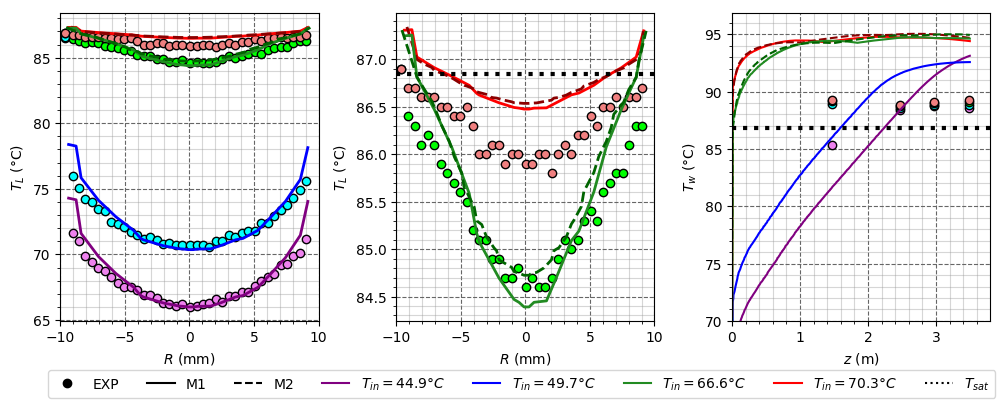
\includegraphics[scale=0.60]{img/DEBORA/c8.png}
\caption{NCFD (lines) vs. Exp. (circles) - $T_{L}$ and $T_{w}$ - Cases C8G2P26W16Te44.9, Te49.6, Te66.6 and Te70.3 - Simulations using two meshes M1 (coarse) and M2 (fine).}
\label{fig:th_1phi_res}
\end{figure}
%

%%
%\begin{figure}[!htb]
%\vspace{16pt}
%\begin{spacing}{1.0}
%\centering
%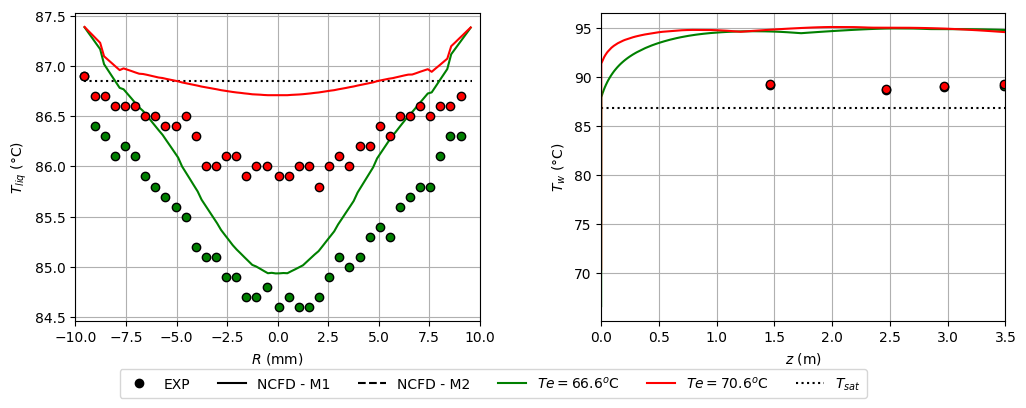
\includegraphics[scale=0.60]{img/DEBORA/thermal_diph.png}
%\caption{NEPTUNE\_CFD simulations results vs. experimental measurements - $T_{L}$ and $T_{w}$ - Cases C8G2P26W16Te66.6 and C8G2P26W16Te70.3}
%\label{fig:th_diph_res}
%\end{spacing}
%\vspace{16pt}
%\end{figure}
%%



%
\begin{figure}[h!]
\centering
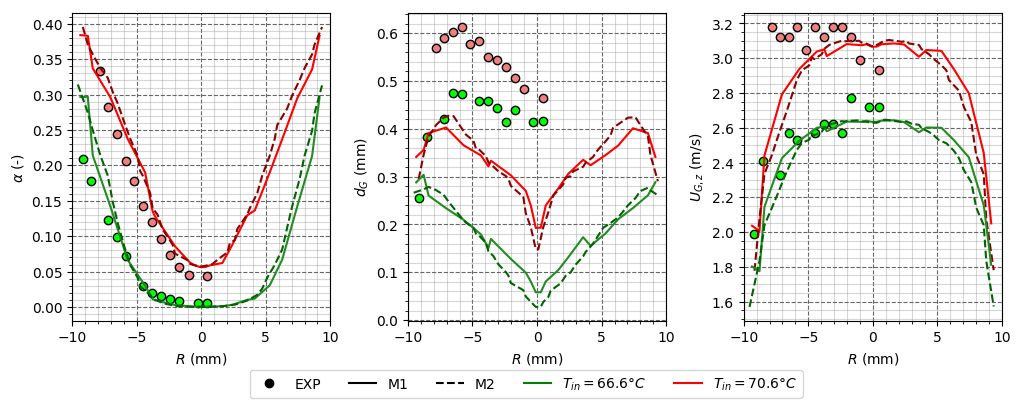
\includegraphics[scale=0.60]{img/DEBORA/c30.png}
\caption{NCFD (lines) vs. Exp. (circles) - $\alpha$, $d_{G}$ and $U_{G,z}$ - Cases C30G2P26W16Te66.6 and Te70.6 - Simulations using two meshes M1 (coarse) and M2 (fine).}
\label{fig:topology_res}
\end{figure}
%

On Figure \ref{fig:topology_res}, we compare the results of the simulations to the experiments regarding void fraction, bubble Sauter diameter and axial gas velocity. Void fraction profiles are quite correctly reproduced, though we observe a $10\%$ higher peak at the wall for $T_{in}=66.6\degree$C. The order of magnitude of bubble diameter is correct ($\sim 0.1\text{mm}$) and NEPTUNE\_CFD manages to detect coalescence (increase of bubble diameter when leaving the wall) and bulk condensation (decrease of bubble diameter when reaching the core of the flow), which is in qualitative agreement with the experiments. Quantitatively speaking, bubble diameter is globally underestimated. Finally, gas velocity profile is reasonably reproduced for $T_{in}=66.6\degree$C, but not for $T_{in}=70.6\degree$C. The latter experimental profile is flatter, which could be explained by a change of flow regime since uncondensed vapor is detected in the bulk.  

Finally, the simulations reasonably agree with the experiments. The strongest discrepancies being mostly the wall temperature and bubble diameter. Potential ways of improving those results are investigated in next sub-section.

\subsection{Investigating the nucleation site density modeling $N_{sit}$}

In NEPTUNE\_CFD, wall temperature is computed through the Heat Flux Partitioning model, which role is to find the appropriate $T_{w}$ which balances Equation $\ref{eq:HFP}$. However, some laws used to express parameters such as $N_{sit}$, $f$, or $d_{d}$ are quite old and simple. For instance, the {Lemmert} \& {Chawla}\cite{Lemmert1977} expression of $N_{sit}$ only depends on the wall superheat (Sub-section \ref{subsec:HFP}).%, meaning that it can not reproduce potential influence of the pressure on the nucleation site density.

A comparison of the {Lemmert} \& {Chawla} law\cite{Lemmert1977} with  the {Hibiki} \& {Ishii}\cite{Hibiki2003} law for $N_{sit}$ against 4 data sets from the literature is presentend on Figure \ref{fig:nsit}. The {Hibiki} \& {Ishii} correlation depends simultaneously on wall superheat, pressure and contact angle.  Experimental measurements of {Borishanskii} \etal\cite{Borishanskii1961}, {Richenderfer} \etal\cite{Richenderfer2018}, {Kossolapov} \etal\cite{Kossolapov2020} and {Zhou} \etal\cite{Zhou2020} are used to assess the two nucleation site density correlations.
%
\begin{figure}[h!]
\centering
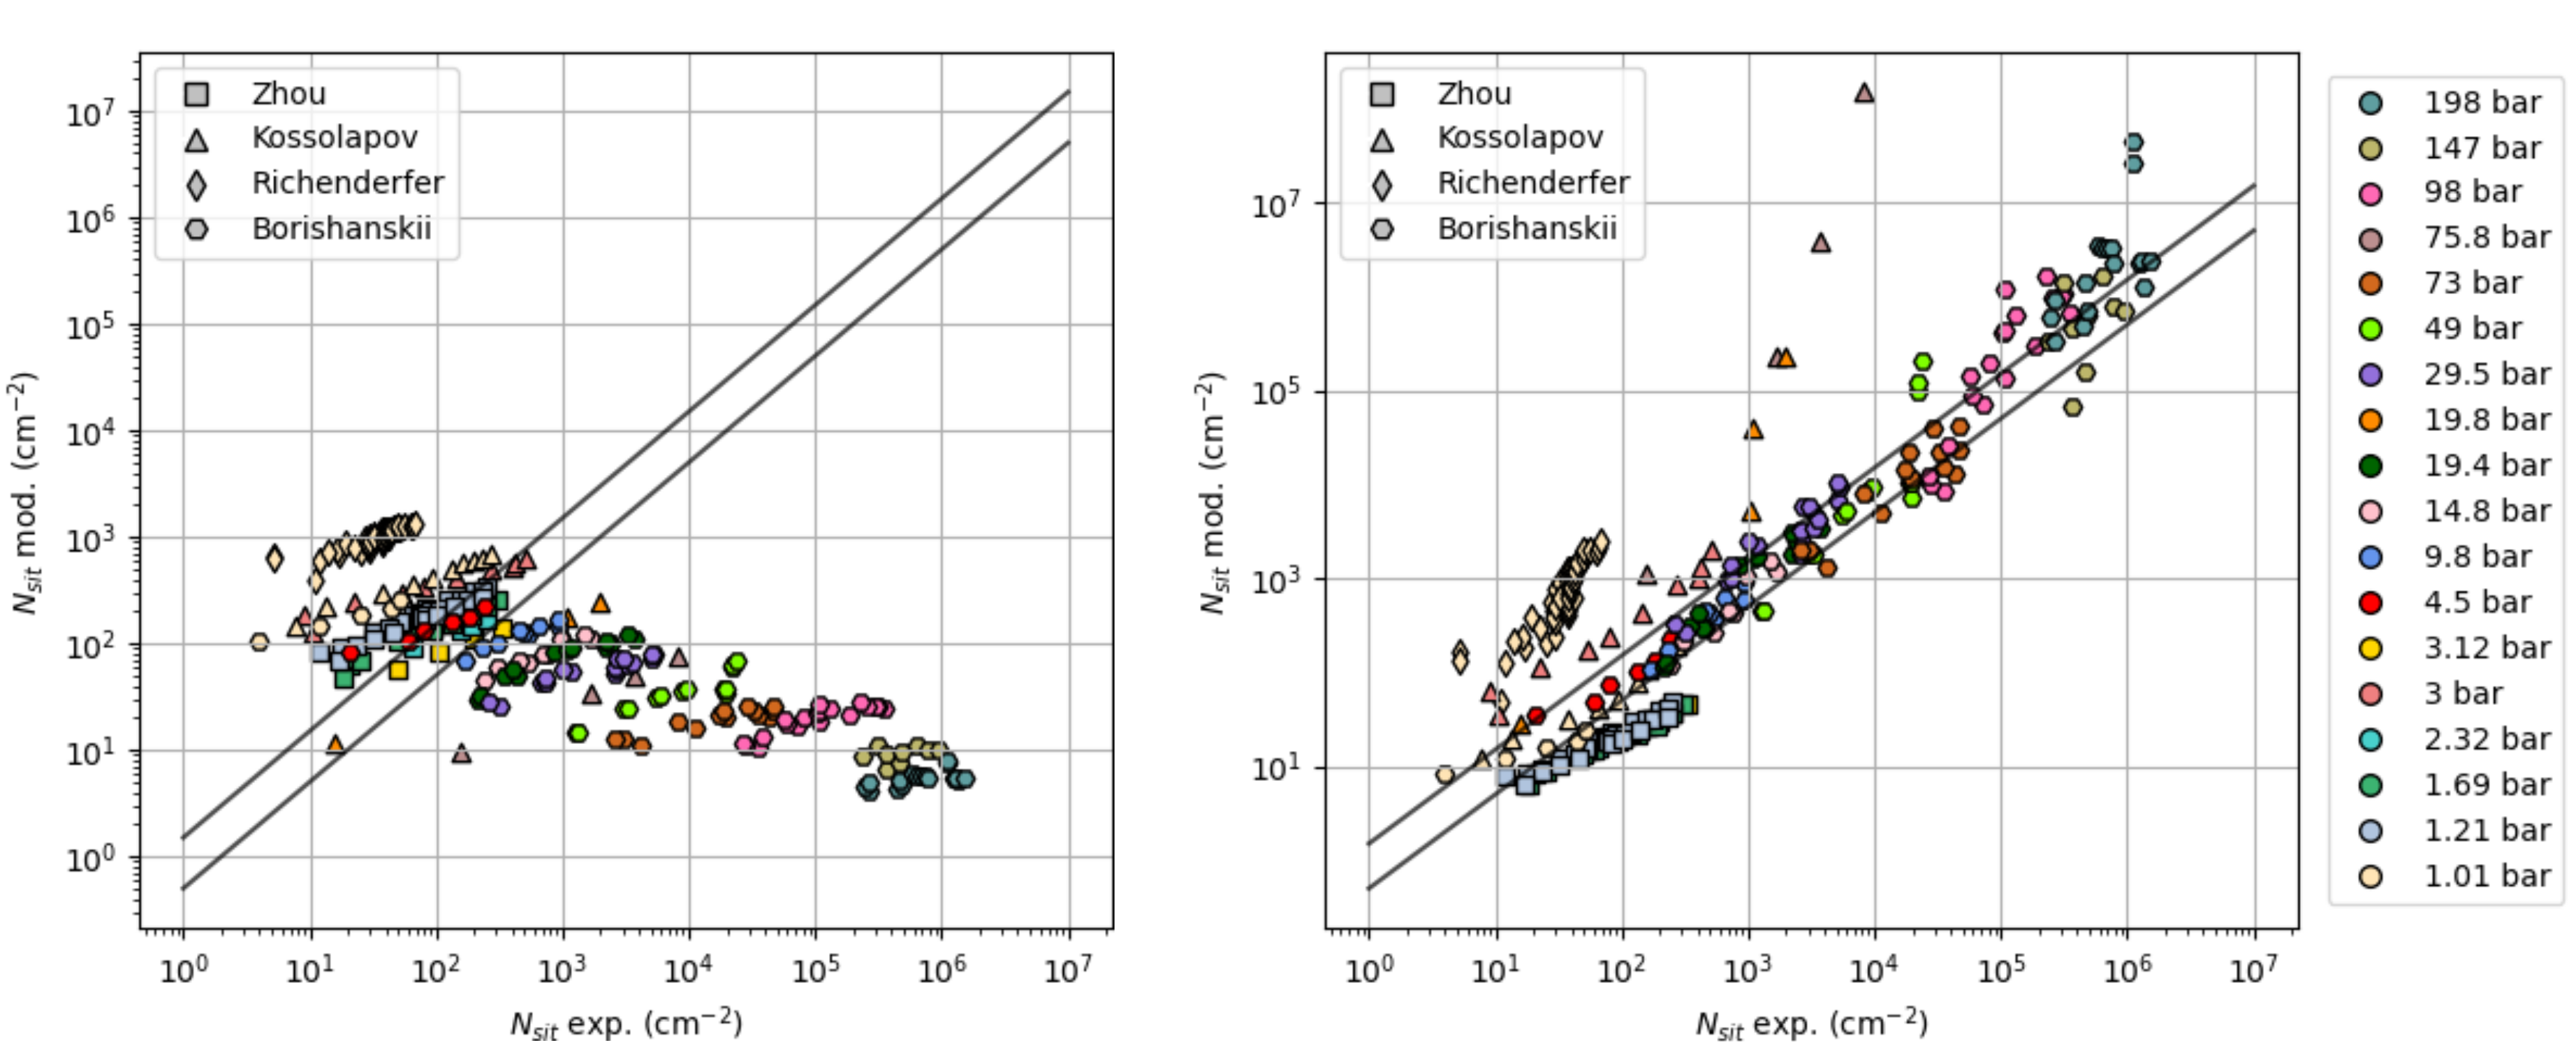
\includegraphics[scale=0.45]{img/DEBORA/nsit.png}
\caption{$N_{sit}$ correlations of {Lemmert} \& {Chawla} (left) and {Hibiki} \& {Ishii} (right) vs. exp. data from literature. Operation pressures are displayed. $\pm 50\%$ error bars are drawn in black.}
\label{fig:nsit}
\end{figure}
%

Figure \ref{fig:nsit} clearly shows that the {Lemmert} \& {Chawla} law lack of pressure dependence fails to reproduce high pressure measurements contrary to the {Hibiki} \& {Ishii} one. Even though {Hibiki} \& {Ishii} correlation shows significant discrepancies with measurements of {Kossolapov} \etal and {Richenderfer} \etal, its prediction capability is greater in average than {Lemmert} \& {Chawla} correlation.

%
\begin{figure}[h!]
\centering
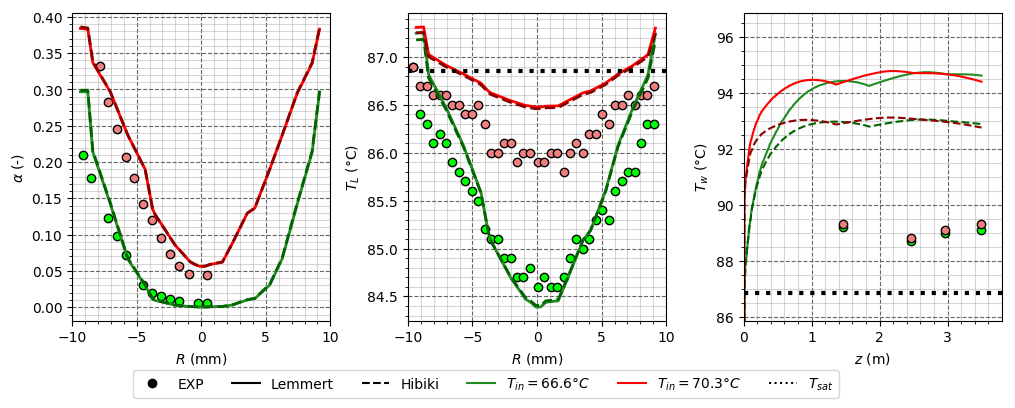
\includegraphics[scale=0.60]{img/DEBORA/plot_HI.png}
\caption{NCFD results for $\alpha$, $T_{L}$ and $T_{w}$ using {Lemmert} \& {Chawla} and {Hibiki} \& {Ishii} correlation. Cases 8G2P26W23Te66.6 and Te70.3, 30G2P26W23Te66.6 and 70.6.}
\label{fig:NCFD_nsit}
\end{figure}
%
To assess the influence of nucleation site density law on NEPTUNE\_CFD computations, we compare results obtained with both correlations on Figure \ref{fig:NCFD_nsit}, which shows a remarkable impact of the modification of $N_{sit}$ correlation. Using {Hibiki} \& {Ishii} correlation reduces the error on $T_{w}$ by approximately $2\degree\text{C}$ while $\alpha$ and $T_{L}$ remain unchanged. This implies that the same heat flux partitioning is found with the two models, but that the pressure dependence of {Hibiki} \& {Ishii} law helped to balance Equation \ref{eq:HFP} using a lower $T_{w}$, thus closer to experimental measurements.

Such a result indicates that the HFP model could be improved through a systematic analysis of each parameter's impact and modeling (bubble departure diameter, detachment frequency, etc.). Assembling a more recent and consistent model could provide better results regarding wall temperature prediction. Models such as the one developed by {Kommajosyula}\cite {Kommajosyula2020} could be interesting to apply for high-pressure flows.


Now that simple tube boiling flow has been assessed through the presented results, next section will focus on the simulation of boiling flow in a tube equipped with a mixing device.% using DEBORA-Promoteur experimental results.